%% bare_conf_compsoc.tex
%% V1.4b
%% 2015/08/26
%% by Michael Shell
%% See:
%% http://www.michaelshell.org/
%% for current contact information.
%%
%% This is a skeleton file demonstrating the use of IEEEtran.cls
%% (requires IEEEtran.cls version 1.8b or later) with an IEEE Computer
%% Society conference paper.
%%
%% Support sites:
%% http://www.michaelshell.org/tex/ieeetran/
%% http://www.ctan.org/pkg/ieeetran
%% and
%% http://www.ieee.org/

%%*************************************************************************
%% Legal Notice:
%% This code is offered as-is without any warranty either expressed or
%% implied; without even the implied warranty of MERCHANTABILITY or
%% FITNESS FOR A PARTICULAR PURPOSE! 
%% User assumes all risk.
%% In no event shall the IEEE or any contributor to this code be liable for
%% any damages or losses, including, but not limited to, incidental,
%% consequential, or any other damages, resulting from the use or misuse
%% of any information contained here.
%%
%% All comments are the opinions of their respective authors and are not
%% necessarily endorsed by the IEEE.
%%
%% This work is distributed under the LaTeX Project Public License (LPPL)
%% ( http://www.latex-project.org/ ) version 1.3, and may be freely used,
%% distributed and modified. A copy of the LPPL, version 1.3, is included
%% in the base LaTeX documentation of all distributions of LaTeX released
%% 2003/12/01 or later.
%% Retain all contribution notices and credits.
%% ** Modified files should be clearly indicated as such, including  **
%% ** renaming them and changing author support contact information. **
%%*************************************************************************


% *** Authors should verify (and, if needed, correct) their LaTeX system  ***
% *** with the testflow diagnostic prior to trusting their LaTeX platform ***
% *** with production work. The IEEE's font choices and paper sizes can   ***
% *** trigger bugs that do not appear when using other class files.       ***                          ***
% The testflow support page is at:
% http://www.michaelshell.org/tex/testflow/



\documentclass[conference,compsoc]{IEEEtran}
% Some/most Computer Society conferences require the compsoc mode option,
% but others may want the standard conference format.
%
% If IEEEtran.cls has not been installed into the LaTeX system files,
% manually specify the path to it like:
% \documentclass[conference,compsoc]{../sty/IEEEtran}





% Some very useful LaTeX packages include:
% (uncomment the ones you want to load)


% *** MISC UTILITY PACKAGES ***
%
%\usepackage{ifpdf}
% Heiko Oberdiek's ifpdf.sty is very useful if you need conditional
% compilation based on whether the output is pdf or dvi.
% usage:
% \ifpdf
%   % pdf code
% \else
%   % dvi code
% \fi
% The latest version of ifpdf.sty can be obtained from:
% http://www.ctan.org/pkg/ifpdf
% Also, note that IEEEtran.cls V1.7 and later provides a builtin
% \ifCLASSINFOpdf conditional that works the same way.
% When switching from latex to pdflatex and vice-versa, the compiler may
% have to be run twice to clear warning/error messages.






% *** CITATION PACKAGES ***
%
\ifCLASSOPTIONcompsoc
  % IEEE Computer Society needs nocompress option
  % requires cite.sty v4.0 or later (November 2003)
  \usepackage[nocompress]{cite}
\else
  % normal IEEE
  \usepackage{cite}
\fi
% cite.sty was written by Donald Arseneau
% V1.6 and later of IEEEtran pre-defines the format of the cite.sty package
% \cite{} output to follow that of the IEEE. Loading the cite package will
% result in citation numbers being automatically sorted and properly
% "compressed/ranged". e.g., [1], [9], [2], [7], [5], [6] without using
% cite.sty will become [1], [2], [5]--[7], [9] using cite.sty. cite.sty's
% \cite will automatically add leading space, if needed. Use cite.sty's
% noadjust option (cite.sty V3.8 and later) if you want to turn this off
% such as if a citation ever needs to be enclosed in parenthesis.
% cite.sty is already installed on most LaTeX systems. Be sure and use
% version 5.0 (2009-03-20) and later if using hyperref.sty.
% The latest version can be obtained at:
% http://www.ctan.org/pkg/cite
% The documentation is contained in the cite.sty file itself.
%
% Note that some packages require special options to format as the Computer
% Society requires. In particular, Computer Society  papers do not use
% compressed citation ranges as is done in typical IEEE papers
% (e.g., [1]-[4]). Instead, they list every citation separately in order
% (e.g., [1], [2], [3], [4]). To get the latter we need to load the cite
% package with the nocompress option which is supported by cite.sty v4.0
% and later.





% *** GRAPHICS RELATED PACKAGES ***
%
\ifCLASSINFOpdf
  \usepackage[pdftex]{graphicx}
  % declare the path(s) where your graphic files are
  \graphicspath{{/home/csj7701/School/2S/Lab2/Lab2 - Copy/}}
  % and their extensions so you won't have to specify these with
  % every instance of \includegraphics
  \DeclareGraphicsExtensions{.pdf,.jpeg,.png}
\else
  % or other class option (dvipsone, dvipdf, if not using dvips). graphicx
  % will default to the driver specified in the system graphics.cfg if no
  % driver is specified.
  \usepackage[dvips]{graphicx}
  % declare the path(s) where your graphic files are
  \graphicspath{{/home/csj7701/School/2S/Lab2/Lab2 - Copy/}}
  % and their extensions so you won't have to specify these with
  % every instance of \includegraphics
  \DeclareGraphicsExtensions{.jpg}
\fi
% graphicx was written by David Carlisle and Sebastian Rahtz. It is
% required if you want graphics, photos, etc. graphicx.sty is already
% installed on most LaTeX systems. The latest version and documentation
% can be obtained at: 
% http://www.ctan.org/pkg/graphicx
% Another good source of documentation is "Using Imported Graphics in
% LaTeX2e" by Keith Reckdahl which can be found at:
% http://www.ctan.org/pkg/epslatex
%
% latex, and pdflatex in dvi mode, support graphics in encapsulated
% postscript (.eps) format. pdflatex in pdf mode supports graphics
% in .pdf, .jpeg, .png and .mps (metapost) formats. Users should ensure
% that all non-photo figures use a vector format (.eps, .pdf, .mps) and
% not a bitmapped formats (.jpeg, .png). The IEEE frowns on bitmapped formats
% which can result in "jaggedy"/blurry rendering of lines and letters as
% well as large increases in file sizes.
%
% You can find documentation about the pdfTeX application at:
% http://www.tug.org/applications/pdftex





% *** MATH PACKAGES ***
%
%\usepackage{amsmath}
% A popular package from the American Mathematical Society that provides
% many useful and powerful commands for dealing with mathematics.
%
% Note that the amsmath package sets \interdisplaylinepenalty to 10000
% thus preventing page breaks from occurring within multiline equations. Use:
%\interdisplaylinepenalty=2500
% after loading amsmath to restore such page breaks as IEEEtran.cls normally
% does. amsmath.sty is already installed on most LaTeX systems. The latest
% version and documentation can be obtained at:
% http://www.ctan.org/pkg/amsmath





% *** SPECIALIZED LIST PACKAGES ***
%
%\usepackage{algorithmic}
% algorithmic.sty was written by Peter Williams and Rogerio Brito.
% This package provides an algorithmic environment fo describing algorithms.
% You can use the algorithmic environment in-text or within a figure
% environment to provide for a floating algorithm. Do NOT use the algorithm
% floating environment provided by algorithm.sty (by the same authors) or
% algorithm2e.sty (by Christophe Fiorio) as the IEEE does not use dedicated
% algorithm float types and packages that provide these will not provide
% correct IEEE style captions. The latest version and documentation of
% algorithmic.sty can be obtained at:
% http://www.ctan.org/pkg/algorithms
% Also of interest may be the (relatively newer and more customizable)
% algorithmicx.sty package by Szasz Janos:
% http://www.ctan.org/pkg/algorithmicx




% *** ALIGNMENT PACKAGES ***
%
%\usepackage{array}
% Frank Mittelbach's and David Carlisle's array.sty patches and improves
% the standard LaTeX2e array and tabular environments to provide better
% appearance and additional user controls. As the default LaTeX2e table
% generation code is lacking to the point of almost being broken with
% respect to the quality of the end results, all users are strongly
% advised to use an enhanced (at the very least that provided by array.sty)
% set of table tools. array.sty is already installed on most systems. The
% latest version and documentation can be obtained at:
% http://www.ctan.org/pkg/array


% IEEEtran contains the IEEEeqnarray family of commands that can be used to
% generate multiline equations as well as matrices, tables, etc., of high
% quality.




% *** SUBFIGURE PACKAGES ***
%\ifCLASSOPTIONcompsoc
%  \usepackage[caption=false,font=footnotesize,labelfont=sf,textfont=sf]{subfig}
%\else
%  \usepackage[caption=false,font=footnotesize]{subfig}
%\fi
% subfig.sty, written by Steven Douglas Cochran, is the modern replacement
% for subfigure.sty, the latter of which is no longer maintained and is
% incompatible with some LaTeX packages including fixltx2e. However,
% subfig.sty requires and automatically loads Axel Sommerfeldt's caption.sty
% which will override IEEEtran.cls' handling of captions and this will result
% in non-IEEE style figure/table captions. To prevent this problem, be sure
% and invoke subfig.sty's "caption=false" package option (available since
% subfig.sty version 1.3, 2005/06/28) as this is will preserve IEEEtran.cls
% handling of captions.
% Note that the Computer Society format requires a sans serif font rather
% than the serif font used in traditional IEEE formatting and thus the need
% to invoke different subfig.sty package options depending on whether
% compsoc mode has been enabled.
%
% The latest version and documentation of subfig.sty can be obtained at:
% http://www.ctan.org/pkg/subfig




% *** FLOAT PACKAGES ***
%
%\usepackage{fixltx2e}
% fixltx2e, the successor to the earlier fix2col.sty, was written by
% Frank Mittelbach and David Carlisle. This package corrects a few problems
% in the LaTeX2e kernel, the most notable of which is that in current
% LaTeX2e releases, the ordering of single and double column floats is not
% guaranteed to be preserved. Thus, an unpatched LaTeX2e can allow a
% single column figure to be placed prior to an earlier double column
% figure.
% Be aware that LaTeX2e kernels dated 2015 and later have fixltx2e.sty's
% corrections already built into the system in which case a warning will
% be issued if an attempt is made to load fixltx2e.sty as it is no longer
% needed.
% The latest version and documentation can be found at:
% http://www.ctan.org/pkg/fixltx2e


%\usepackage{stfloats}
% stfloats.sty was written by Sigitas Tolusis. This package gives LaTeX2e
% the ability to do double column floats at the bottom of the page as well
% as the top. (e.g., "\begin{figure*}[!b]" is not normally possible in
% LaTeX2e). It also provides a command:
%\fnbelowfloat
% to enable the placement of footnotes below bottom floats (the standard
% LaTeX2e kernel puts them above bottom floats). This is an invasive package
% which rewrites many portions of the LaTeX2e float routines. It may not work
% with other packages that modify the LaTeX2e float routines. The latest
% version and documentation can be obtained at:
% http://www.ctan.org/pkg/stfloats
% Do not use the stfloats baselinefloat ability as the IEEE does not allow
% \baselineskip to stretch. Authors submitting work to the IEEE should note
% that the IEEE rarely uses double column equations and that authors should try
% to avoid such use. Do not be tempted to use the cuted.sty or midfloat.sty
% packages (also by Sigitas Tolusis) as the IEEE does not format its papers in
% such ways.
% Do not attempt to use stfloats with fixltx2e as they are incompatible.
% Instead, use Morten Hogholm'a dblfloatfix which combines the features
% of both fixltx2e and stfloats:
%
% \usepackage{dblfloatfix}
% The latest version can be found at:
% http://www.ctan.org/pkg/dblfloatfix




% *** PDF, URL AND HYPERLINK PACKAGES ***
%
%\usepackage{url}
% url.sty was written by Donald Arseneau. It provides better support for
% handling and breaking URLs. url.sty is already installed on most LaTeX
% systems. The latest version and documentation can be obtained at:
% http://www.ctan.org/pkg/url
% Basically, \url{my_url_here}.




% *** Do not adjust lengths that control margins, column widths, etc. ***
% *** Do not use packages that alter fonts (such as pslatex).         ***
% There should be no need to do such things with IEEEtran.cls V1.6 and later.
% (Unless specifically asked to do so by the journal or conference you plan
% to submit to, of course. )


% correct bad hyphenation here
\hyphenation{op-tical net-works semi-conduc-tor}
\graphicspath{ {/home/csj7701/School/2S/Controls/Lab2/Lab2 - Copy/} }

\begin{document}
%
% paper title
% Titles are generally capitalized except for words such as a, an, and, as,
% at, but, by, for, in, nor, of, on, or, the, to and up, which are usually
% not capitalized unless they are the first or last word of the title.
% Linebreaks \\ can be used within to get better formatting as desired.
% Do not put math or special symbols in the title.
\title{First Order System Identification and Real Time DC Motor Modeling\\Automatic Control Systems (1331)  -  Lab 3}


% author names and affiliations
% use a multiple column layout for up to three different
% affiliations
\author{\IEEEauthorblockN{Christian Johnson}
\IEEEauthorblockA{Electrical Engineering Department\\
United States Coast Guard Academy\\
New London, Connecticut 06320\\
Email: Christian.S.Johnson@uscga.edu}
\and
\IEEEauthorblockN{Riley Thorburn}
\IEEEauthorblockA{Electrical Engineering Department\\
New London, Connecticut 06320\\
Email: Riley.S.Thorburn@uscga.edu}}

% conference papers do not typically use \thanks and this command
% is locked out in conference mode. If really needed, such as for
% the acknowledgment of grants, issue a \IEEEoverridecommandlockouts
% after \documentclass

% for over three affiliations, or if they all won't fit within the width
% of the page (and note that there is less available width in this regard for
% compsoc conferences compared to traditional conferences), use this
% alternative format:
% 
%\author{\IEEEauthorblockN{Michael Shell\IEEEauthorrefmark{1},
%Homer Simpson\IEEEauthorrefmark{2},
%James Kirk\IEEEauthorrefmark{3}, 
%Montgomery Scott\IEEEauthorrefmark{3} and
%Eldon Tyrell\IEEEauthorrefmark{4}}
%\IEEEauthorblockA{\IEEEauthorrefmark{1}School of Electrical and Computer Engineering\\
%Georgia Institute of Technology,
%Atlanta, Georgia 30332--0250\\ Email: see http://www.michaelshell.org/contact.html}
%\IEEEauthorblockA{\IEEEauthorrefmark{2}Twentieth Century Fox, Springfield, USA\\
%Email: homer@thesimpsons.com}
%\IEEEauthorblockA{\IEEEauthorrefmark{3}Starfleet Academy, San Francisco, California 96678-2391\\
%Telephone: (800) 555--1212, Fax: (888) 555--1212}
%\IEEEauthorblockA{\IEEEauthorrefmark{4}Tyrell Inc., 123 Replicant Street, Los Angeles, California 90210--4321}}




% use for special paper notices
%\IEEEspecialpapernotice{(Invited Paper)}




% make the title area
\maketitle

% As a general rule, do not put math, special symbols or citations
% in the abstract
\begin{abstract}
The abstract goes here.
\end{abstract}

% no keywords




% For peer review papers, you can put extra information on the cover
% page as needed:
% \ifCLASSOPTIONpeerreview
% \begin{center} \bfseries EDICS Category: 3-BBND \end{center}
% \fi
%
% For peerreview papers, this IEEEtran command inserts a page break and
% creates the second title. It will be ignored for other modes.
\IEEEpeerreviewmaketitle



\section{Introduction}
DC Motors are an integral part of our daily life. Offering precise control and actuation, they are typically used in transportation, consumer electronics, medical devices, and heavy machinery. Within the United States Coast Guard (USCG), DC motors play a crucial role, not only in propulsion systems for cutters and small boats, but also in smaller auxiliary tasks. From powering pulley systems used in helicopter operations to winches used in lowering small-boats from a boat deck, DC motors form the backbone of many critical operations within the USCG.

This laboratory experiment served as an exploration into the function and control of basic DC motors, particularly focusing on the SRV02 DC motor system. Delving into the principles of automatic control systems, this experiment aimed to provide students with practical insights into system identification, verification, and validation processes. Through hands on experimentation and analysis, students gained a deeper understanding of how to model and analyze the dynamic behavior of such systems, preparing them for future challenges in engineering and control system design.

Building upon the foundation of theoretical knowledge and real world applications, this lab aimed to bridge the gap between classroom learning and practical implementation; empowering students with the skills necessary to tackle complex engineering problems in the field of automatic control systems.
\section{Theory}
In this lab, modeling software enabled us to visualize the behavior of a hardware motor. A SRV02 DC motor can be modeled as a continuous-time transfer function, obtained from measured and simulated motor speed. A transfer function is a mathematical model of linear, time-invariant electrical, mechanical, and electromechanical systems; it is generally defined as $G(s)=\frac{C(s)}{R(s)}$. Referenced throughout this report, $\Omega(s)$ is defined as the angular velocity, $V(s)$ represents the motor input voltage, $K$ denotes the system gains, and $T$ signifies the time constant. These estimations were found using a modeling process reliant on QUARC software and Matlab.

One of the primary problems identified and solved within this lab was the practical estimation of $K$ and $\tau$, which play important roles in the dynamic response of the motor. Solving this problem, and finding values for $K$ and $\tau$ requires a multi-step process. The first step in this process involved the steady-state gain; found by running the system with constant input voltage. Adjusting the system parameters in the given Simulink file helped approximate a frequency close to zero; which, once compiled and applied to the SRV02 motor, began rotating in a single direction, capturing graphs of the motors speed in Matlab. In the figure, the yellow trace represents measured speed, while blue represents simulated speed. This process was repeated twice in order to calculate and record a reliable average.

Through careful analysis, this data helped calculate the steady-state gain. This gain serves as a fundamental parameter in understanding motor performance and behavior. The next step to this analysis process, calculating frequency response, required us to apply a sine wave input, iterating through a range of frequency inputs in order to calculate the resulting range of amplitudes. Using Matlab to analyze this data, we generated a bode magnitude plot from the maximum speed and gain, analyzing this plot in order to find cutoff frequency and $\tau$. Finally, altering the input waveform to a square wave, we applied a step input to the system, measuring shaft speed as system output. This is known as the bump test, and the resulting graph of input and output signals provided the final data we needed in order to calculate $K$ and $\tau$. 

\section{Results}

\subsection{Frequency Response}
The first component of the experiment involved applying sine wave inputs to the SRV02 DC motor and recording the corresponding output speed at varying frequencies. This data was used to construct bode magnitude plots. These plots are shown below.

\begin{figure}[!t]
  \centering
  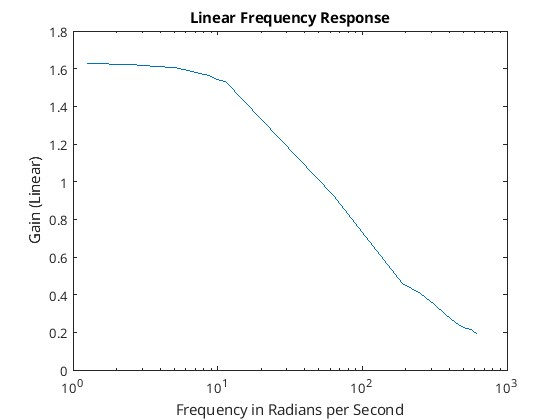
\includegraphics[width=2.5in]{LinearFrequencyResponse.jpg}
  \caption{Linear Frequency Response over a range of frequencies}
  \label{fig_sim}
\end{figure}

\begin{figure}[!t]
  \centering
  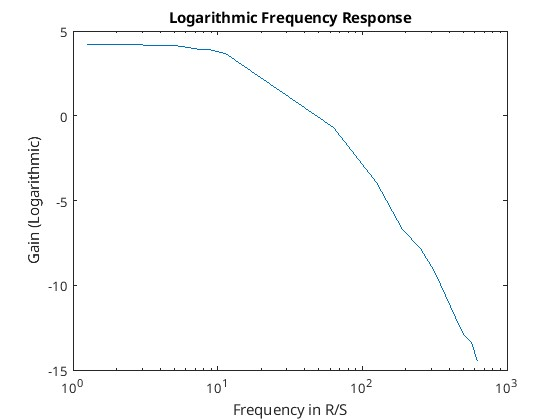
\includegraphics[width=2.5in]{LogFrequencyResponse.jpg}
  \caption{Logarithmic Frequency Response over a range of frequencies}
  \label{fig_sim}
\end{figure}

Using these bode plots and equation 1 below, the steady state gain of the system was found to be in a range between 1.6276 and 0.18855 in linear units, and between 4.2311 and -14.4915 in logarithmic.
\begin{equation}
  K_{e,f}=:|G(j\omega)=|\frac{\Omega_{max-avg}(j\omega)}{V_m(j\omega)}|
\end{equation}
$\tau$ was found visually to be 0.0024 for both linear and logarithmic plots. These values are extrapolated directly from the bode plot, which visualizes the frequency at which the gain begins to decrease, and the phase begins to shift.

\subsection{Step Response}

The next portion of the experiment involved applying a step input voltage to the SRV02 DC motor and recording the corresponding shaft speed, organizing the data into a step response plot. Using Matlab, the step response plot is transformed into the time response.
\begin{equation}
  K_{e,b}=\frac{\delta y}{\delta u}=:\frac{y_{ss}-y{0}}{u_{max}-u_{min}}
\end{equation}
\begin{equation}
  y(t_{1})=0.63y_{ss}+y_{0}
\end{equation}
\begin{equation}
  \tau_{e,b}=t_{1}-t_{0}
\end{equation}

System gain can be calculated from equation 2 above, and utilizing Matlab's \textit{ginput} function, we can find inputs to equations 3 and 4 in order to calculate $\tau$.
From these equations, the average gain was calculated as 1.68805, and the average time constant was found to be 0.04035. These values were found using the overshoot, settling time, and overall response characteristics of the step response plot.

\subsection{Validation and Verification}
Using the information gathered so far, we were able to form a theoretical transfer function for the motor from the frequency and step response. Compating the experimental steady state gain and time constant with the experimental values showed a relatively strong similarity between the two calculations, finding $K$ to be 1.528 and $\tau$ to be 0.0252, which produces a transfer function of $\frac{1.528}{0.0252s+1}$, compared to the results in part one and part two of this experiment.

Following this exercise, we sought to validate the simulated models performance, comparing its results to those we received from the physical system. In order to accomplish this, we first implemented the values calculated in the previous step, then we adjusted the model parameters based on experimental data in order to improve the simulation's accuracy. Using the nominal values calculate in the verification step, we generated the following graph, shown in figure 3.
\begin{figure}[!t]
  \centering
  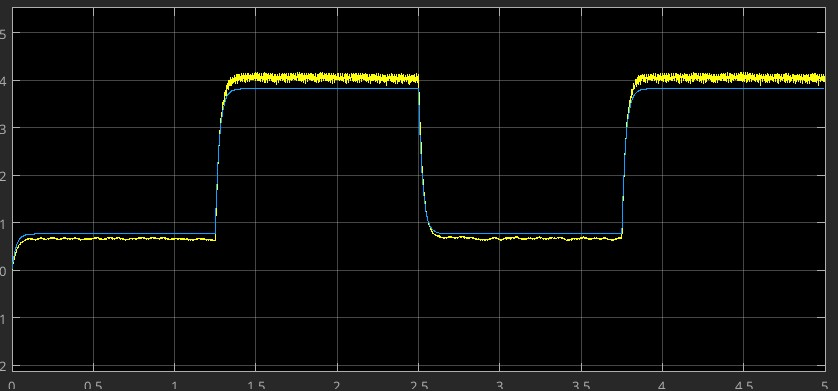
\includegraphics[width=2.5in]{NominalFrequencyResponse.jpg}
  \caption{Nominal Frequency Response}
  \label{fig_sim}
\end{figure}
In figure 3, it is evident that, although the two graphs are quite similar, there is a small variation in amplitude. Factors that contribute to this difference may potentially include friction, physical imperfections in the machine itself (such as wear and tear or manufacturing imperfections), or general imperfections.
Next,we began adjusting variables in an attempt to reduce the difference between the two graphs. Performing this adjustment iteratively, we compared the response plots of the simulated and physical systems, seeking to match them as closely as possible. Figure 4 shows the final result of this process, and demonstrates a remarkeably close match between the simulated and physical system.
\begin{figure}[!t]
  \centering
  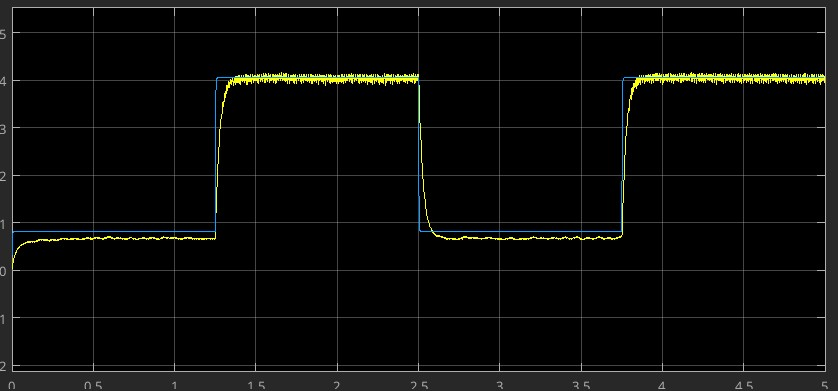
\includegraphics[width=2.5in]{AdjustedFrequencyResponse.jpg}
  \caption{Adjusted Frequency Response}
  \label{fig_sim}
\end{figure}
Using a $K$ of 1.6 and a $\tau$ of 0.0252, the adjusted simulation parameters resulted in a response that matched the experimental response almost exactly. This demonstrates the efficacy of our simulation and experimental process.

\section{Conclusion}
Through this experimental investigatin into steady state gain, frequency response, and step response, we have improved our insight into the SRV02 DC motor and its dynamic response. More specifically, analyzing bode magnitude plots allowed us to determine the gain ($K$) and time constant ($\tau$) for step and frequency responses. Comparing these values to the values we obtained mathematically and those from the simulated model, we attempted to determine the accuracy of our experimental techniques.
This experiment was not without numerous difficulties and challenges. We struggled to properly interpret our bode plots, on several occasions selecting the incorrect location on the plot and therefore obtaining incorrect values. These mistakes emphasized the importance of situational awareness when running experimental simulations.
Overall, the results we obtained from this series of experiments demonstrate the performance and response of the SRV02 motor, and the general effectiveness of the modeling techniques used throughout this procedure; the similarity between the theoretical predictions and experimental observations highlighting the efficacy and reliability of our modeling technique. THese finding have important implications for the design and analysis of control systems in various engineering applications, and will assist us as we explore similar systems within the United States Coast Guard and its many missions. 

% An example of a floating figure using the graphicx package.
% Note that \label must occur AFTER (or within) \caption.
% For figures, \caption should occur after the \includegraphics.
% Note that IEEEtran v1.7 and later has special internal code that
% is designed to preserve the operation of \label within \caption
% even when the captionsoff option is in effect. However, because
% of issues like this, it may be the safest practice to put all your
% \label just after \caption rather than within \caption{}.
%
% Reminder: the "draftcls" or "draftclsnofoot", not "draft", class
% option should be used if it is desired that the figures are to be
% displayed while in draft mode.
%
%\begin{figure}[!t]
%\centering
%\includegraphics[width=2.5in]{myfigure}
% where an .eps filename suffix will be assumed under latex, 
% and a .pdf suffix will be assumed for pdflatex; or what has been declared
% via \DeclareGraphicsExtensions.
%\caption{Simulation results for the network.}
%\label{fig_sim}
%\end{figure}

% Note that the IEEE typically puts floats only at the top, even when this
% results in a large percentage of a column being occupied by floats.


% An example of a double column floating figure using two subfigures.
% (The subfig.sty package must be loaded for this to work.)
% The subfigure \label commands are set within each subfloat command,
% and the \label for the overall figure must come after \caption.
% \hfil is used as a separator to get equal spacing.
% Watch out that the combined width of all the subfigures on a 
% line do not exceed the text width or a line break will occur.
%
%\begin{figure*}[!t]
%\centering
%\subfloat[Case I]{\includegraphics[width=2.5in]{box}%
%\label{fig_first_case}}
%\hfil
%\subfloat[Case II]{\includegraphics[width=2.5in]{box}%
%\label{fig_second_case}}
%\caption{Simulation results for the network.}
%\label{fig_sim}
%\end{figure*}
%
% Note that often IEEE papers with subfigures do not employ subfigure
% captions (using the optional argument to \subfloat[]), but instead will
% reference/describe all of them (a), (b), etc., within the main caption.
% Be aware that for subfig.sty to generate the (a), (b), etc., subfigure
% labels, the optional argument to \subfloat must be present. If a
% subcaption is not desired, just leave its contents blank,
% e.g., \subfloat[].


% An example of a floating table. Note that, for IEEE style tables, the
% \caption command should come BEFORE the table and, given that table
% captions serve much like titles, are usually capitalized except for words
% such as a, an, and, as, at, but, by, for, in, nor, of, on, or, the, to
% and up, which are usually not capitalized unless they are the first or
% last word of the caption. Table text will default to \footnotesize as
% the IEEE normally uses this smaller font for tables.
% The \label must come after \caption as always.
%
%\begin{table}[!t]
%% increase table row spacing, adjust to taste
%\renewcommand{\arraystretch}{1.3}
% if using array.sty, it might be a good idea to tweak the value of
% \extrarowheight as needed to properly center the text within the cells
%\caption{An Example of a Table}
%\label{table_example}
%\centering
%% Some packages, such as MDW tools, offer better commands for making tables
%% than the plain LaTeX2e tabular which is used here.
%\begin{tabular}{|c||c|}
%\hline
%One & Two\\
%\hline
%Three & Four\\
%\hline
%\end{tabular}
%\end{table}


% Note that the IEEE does not put floats in the very first column
% - or typically anywhere on the first page for that matter. Also,
% in-text middle ("here") positioning is typically not used, but it
% is allowed and encouraged for Computer Society conferences (but
% not Computer Society journals). Most IEEE journals/conferences use
% top floats exclusively. 
% Note that, LaTeX2e, unlike IEEE journals/conferences, places
% footnotes above bottom floats. This can be corrected via the
% \fnbelowfloat command of the stfloats package.




\section{Conclusion}
The conclusion goes here.




% trigger a \newpage just before the given reference
% number - used to balance the columns on the last page
% adjust value as needed - may need to be readjusted if
% the document is modified later
%\IEEEtriggeratref{8}
% The "triggered" command can be changed if desired:
%\IEEEtriggercmd{\enlargethispage{-5in}



% that's all folks
\end{document}
